\section{Introduction}
\label{Sec:Introduction}
 
 Given a point $\mu$ in a normed linear space $\cX$ with norm denoted by $| \cdot |$, 
 the \textit{generalized sign function} 
 $S : \cX \times \cX \mapsto \cX$ with center $\mu$ is  
 defined as
\baq
S (x; \mu) =  \left\{ 
\begin{array}{ll}
| x - \mu|^{-1} ( x - \mu ) &  \text{ if } x \ne \mu, \\
0 & \text{ if } x = \mu.
\end{array}
\right.
\label{eq:GSign}
\eaq
This is a functional and multivariate  generalization of the real-valued 
\textit{sign function}, that 
takes the values one, negative one or zero if the point $x \in \BR$ is to the right, left 
or equal $\mu \in \BR$ respectively. This generalized sign function was  
introduced by \cite{ref:JNonpara95201_MottonenOja95} for $\cX = \BR^{p}$, 
the $p$-dimensional  real Euclidean space. 


The function $S$ maps $\mu$ to the origin and all other points of $\cX$ 
to the unit sphere  ${\cS}_{0; 1} = \{ x \in \cX: | x | = 1 \}$. 
Given a dataset  $\{ X_{i} \in \BR^{p}: i =1, \ldots, n \}$,
that we collect together in 
the $n \times p$ matrix $\bfX = ( X_{1}: \ldots : X_{n} )^{T}$,
an approach for robust estimation and inference in multivariate data starts by evaluating  
\eqref{eq:GSign} on each observation, thus defining 
$S_{i} = S ( X_{i}; \mu_x)$ with respect to some suitable center 
$ \mu_x \in \BR^{p}$, and then using these for robust location and scale estimation and 
inference, including inference for $ \mu_x$ 
\citep{ref:Test991_Locantoreetal, ref:OjaBook10, ref:JASA151658_WangPengLi}.
Suppose $\bfS = ( S_{1}: \ldots : S_{n} )^{T} \in \BR^{n \times p}$. 
If the data $\{ X_{i} \in \BR^{p}: i =1, \ldots, n \}$ are independent, identically 
distributed (hereafter, i.i.d.) from an elliptically symmetric distribution, then the 
eigenvectors of $\BE ( X_{1} - \tilde{\mu}) ( X_{1} - \tilde{\mu})^{T}$
and of $\BE S_{1} S_{1}^{T}$ are the same for suitable centering 
parameters $\tilde{\mu}$ and $ \mu_x$, that is, the population principal components 
from the original data and from its sign transformations are the same 
\citep{ref:SPL12765_Taskinenetal}. However, valuable information is lost in the form of magnitudes of sample points. As a result, spatial sign-based procedures suffer from low efficiency. For example, eigenvector estimates obtained from the covariance matrix of $S$ are asymptotically inadmissible \citep{ref:Biometrika14673_MagyarTyler} and  Tyler's M-estimate of scatter \citep{ref:AoS87234_Tyler} has uniformly lower asymptotic risk. 

In this paper, we propose to alleviate this low efficiency problem, by associating 
a data-driven weight $W_{i}$ with the generalized sign $S_{i}$, that can be used 
to adaptively trade-off between efficiency and robustness considerations in any given 
application. We demonstrate the utility of using the proposed \textit{weighted generalized sign} functions in a number of problems of current interest, including robust estimation of location and scatter.

Specifically, we propose using product of the generalized sign function and a weight function derived as a transformation of a data-depth function \citep{ref:DIMACS061_Serfling, ref:AoS00461_ZuoSerfling}. Like data-depth functions, the weight functions used in this paper are non-negative reals defined over $\cX \times \cF$, where $\cF$ is a fixed family of probability measures. For every choice of parameters $\mu \in \cX$ and $\BF \in \cF$, in this paper
%
\begin{align}
R (X_{i}; \mu, \BF) = \mu +  S( X_{i}, \mu) W( X_{i}, \BF).
\label{eqn:rank}
\end{align}
%
is used as a robust surrogate for observation $X_{i}$.
Notice that for the trivial choice $W( x, \BF) = | x - \mu_{\BF} |$, 
 $\mu = \mu_{\BF}$,  we get $R (X_{i}; \mu, \BF) = X_{i}$, the original observations. 
 With the other trivial choice of  $W( x, \BF) \equiv 1$, we get the 
 generalized  sign $R (X_{i}; \mu, \BF) = S(X_{i}, \mu) = S_{i}$. 
 However, in this paper we illustrate how using other weight functions
 can lead to interesting robustness and efficiency trade-offs in a variety of situations. 
 The various technical conditions and assumptions that we impose on the 
 weight function $W( x, \BF)$ are valid for weights derived 
 from three well-known data depth functions: the \textit{half-space depth}, 
 the \textit{Mahalanobis depth}, and the \textit{projection depth}. Note that for i.i.d. data, there are three parameters involved here: the location parameter $\mu$ in 
 \eqref{eq:GSign}, the distribution $\BF$ used for the weight function, and the distribution $\BF_{X}$ of $X_{1}$. For clarity and to mirror the contexts of how data depth has been used in the literature \cite{LiuPareliusSingh99, ref:DIMACS061_Serfling}, we fix $\BF = \BF_{X}$ for this paper, although in Section~\ref{Sec:WSQuantiles} we briefly remark on the case when these  distributions are different. Also note that 
 in many problems of interest, $\BF$ is 
unknown and  data-depths are computed using $\BF_{n}$, however, under very standard regularity conditions (for example, see assumptions \textbf{B1-B3} below), the 
properties of $W (x, \BF)$ and $W (x, \BF_{n})$ are close enough for both asymptotic theory and practical applicability.  
 
 %\begin{comment}
\begin{figure}[t!]
%\captionsetup{justification=centering, font=footnotesize}
\begin{center}
%\begin{tabular}{ll}
%%% These ones have sample size = 700, just right  for EJS
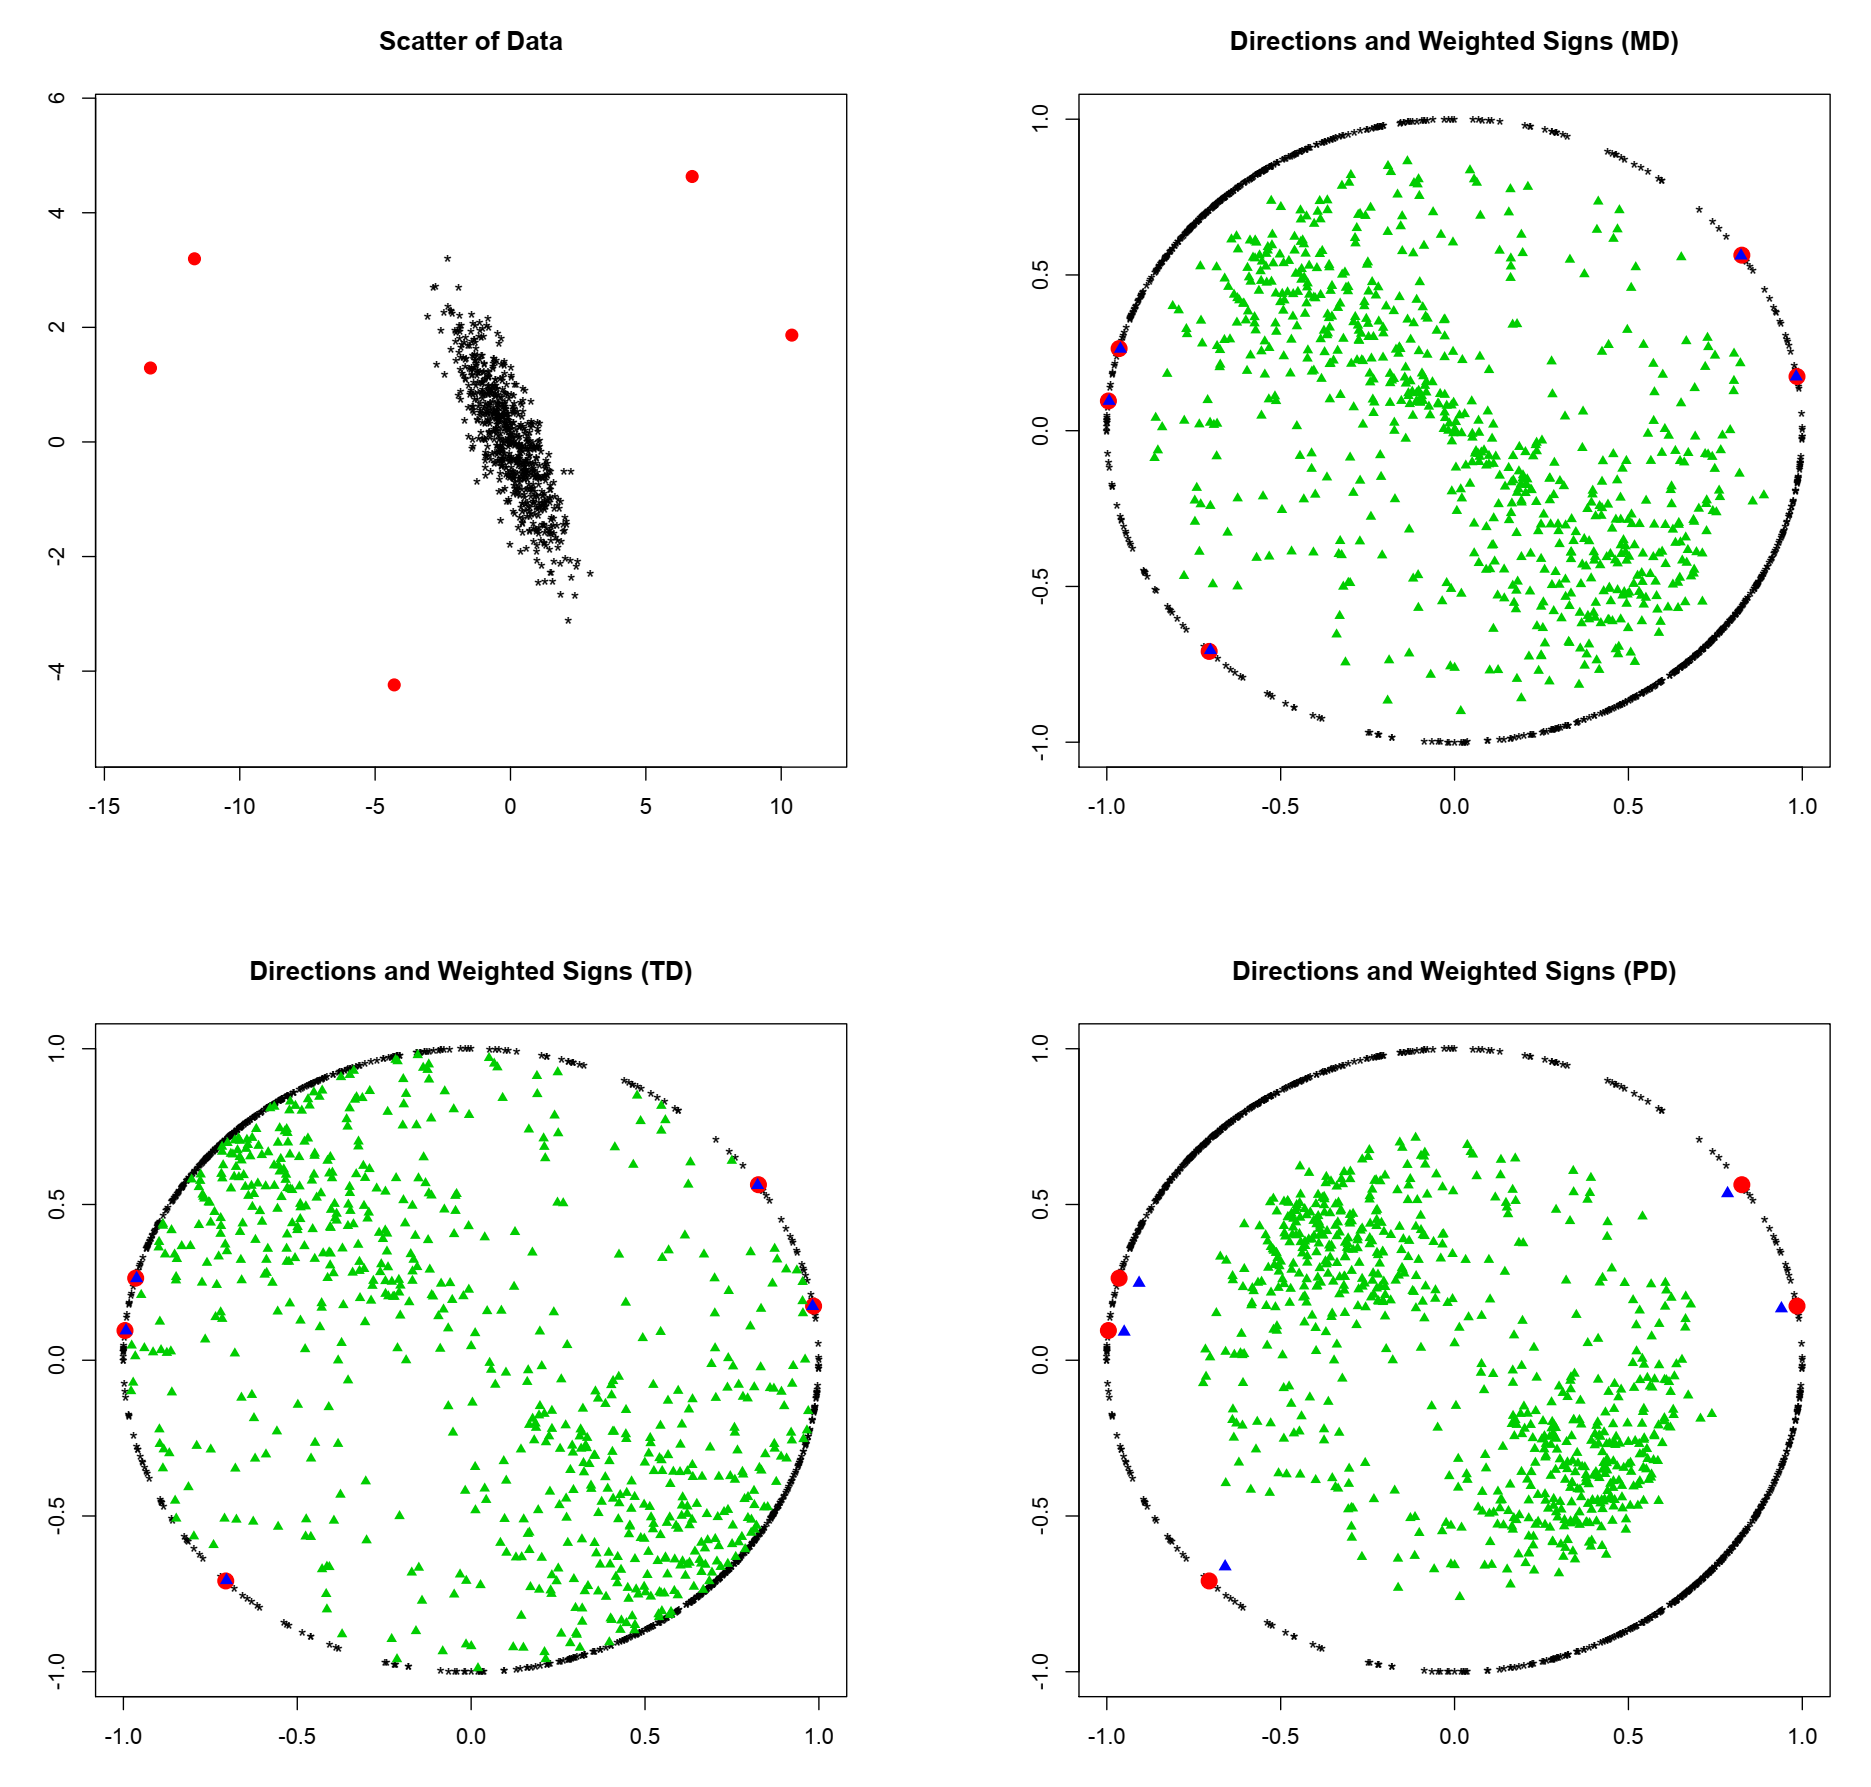
\includegraphics[width=\textwidth]{./Plots/WeightedSignAll}
%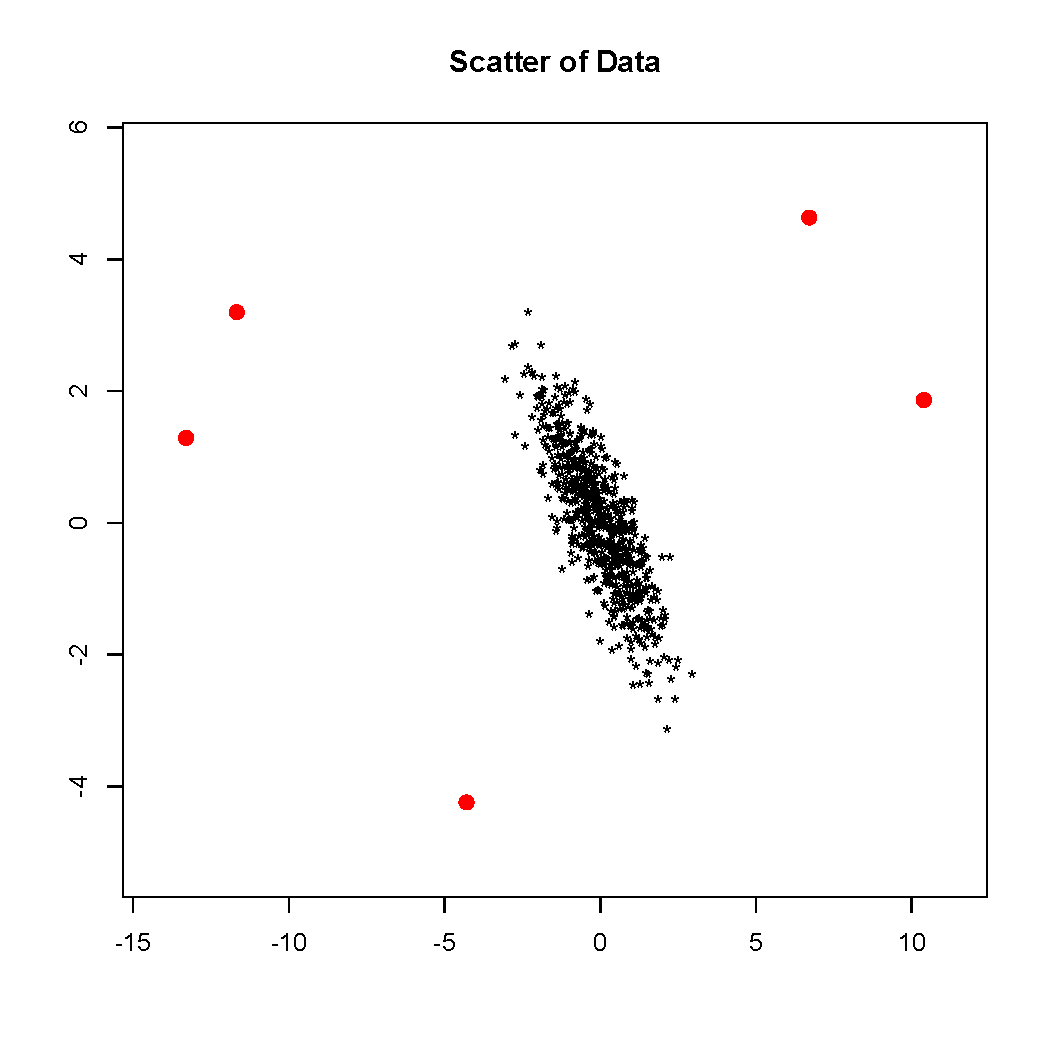
\includegraphics[width=0.45\textwidth]{./Plots_SC/WeightedSign_Scatter_700_02_27_19} &
%\includegraphics[width=0.45\textwidth]{./Plots_SC/WeightedSign_MD_700_02_27_19} \\
%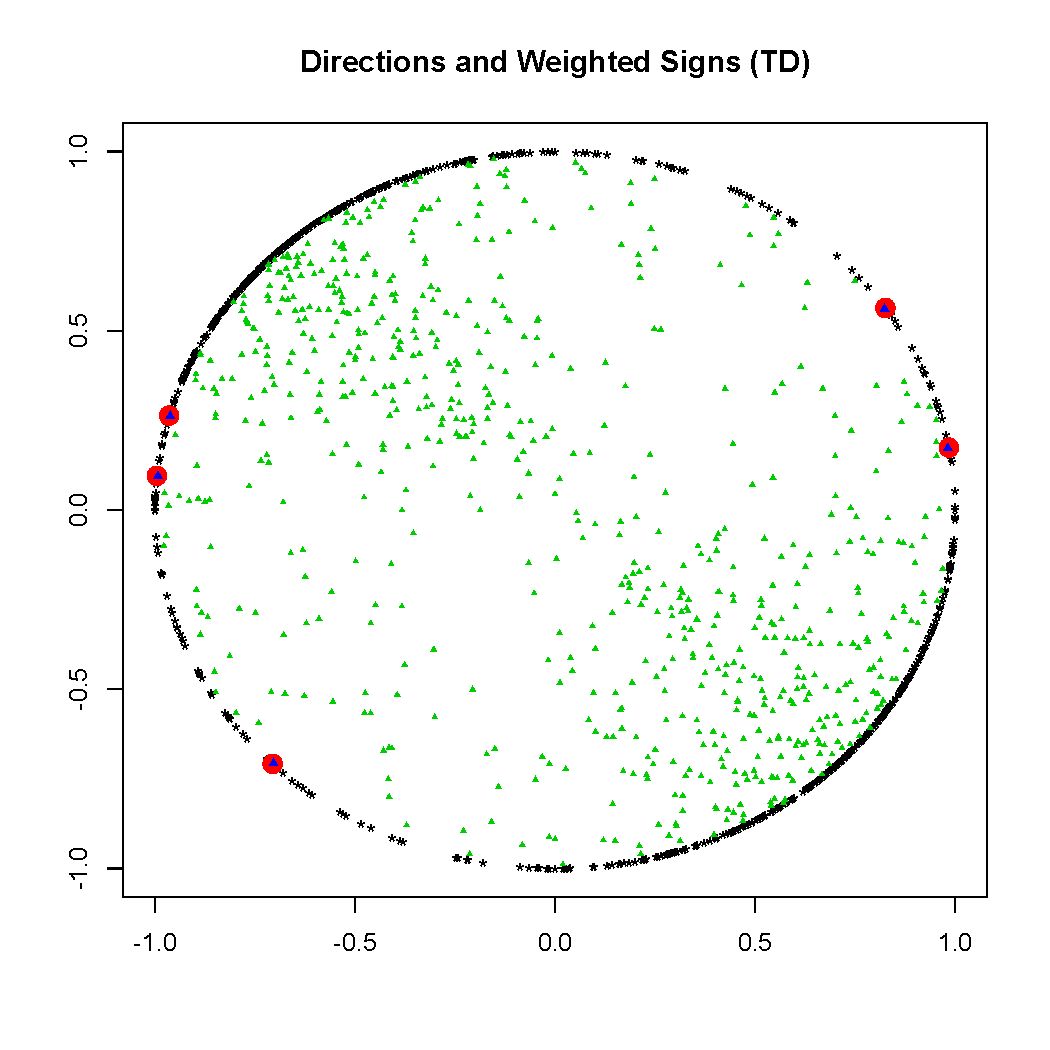
\includegraphics[width=0.45\textwidth]{./Plots_SC/WeightedSign_TD_700_02_27_19} &
%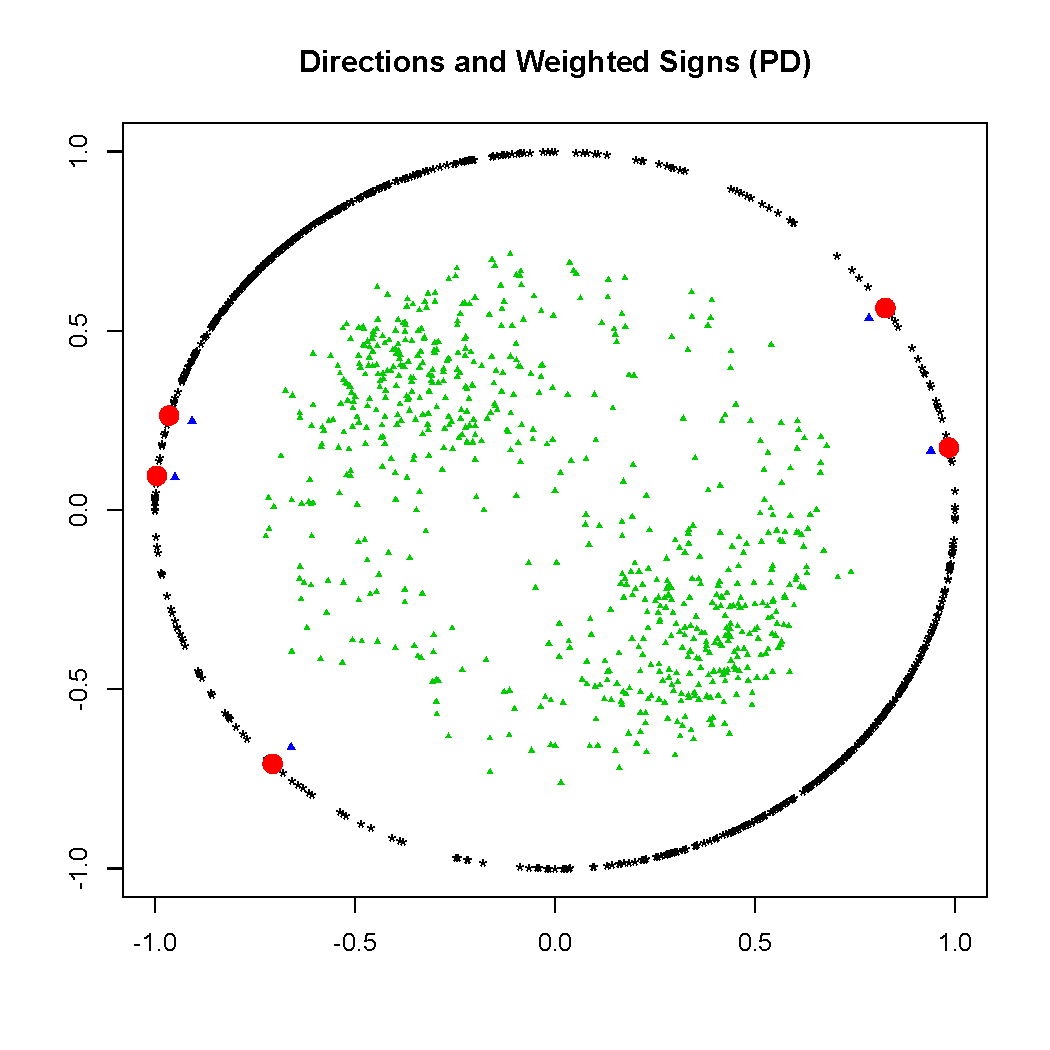
\includegraphics[width=0.45\textwidth]{./Plots_SC/WeightedSign_PD_700_02_27_19} \\

%%% These ones have sample size = 300, OK but too small file for EJS
%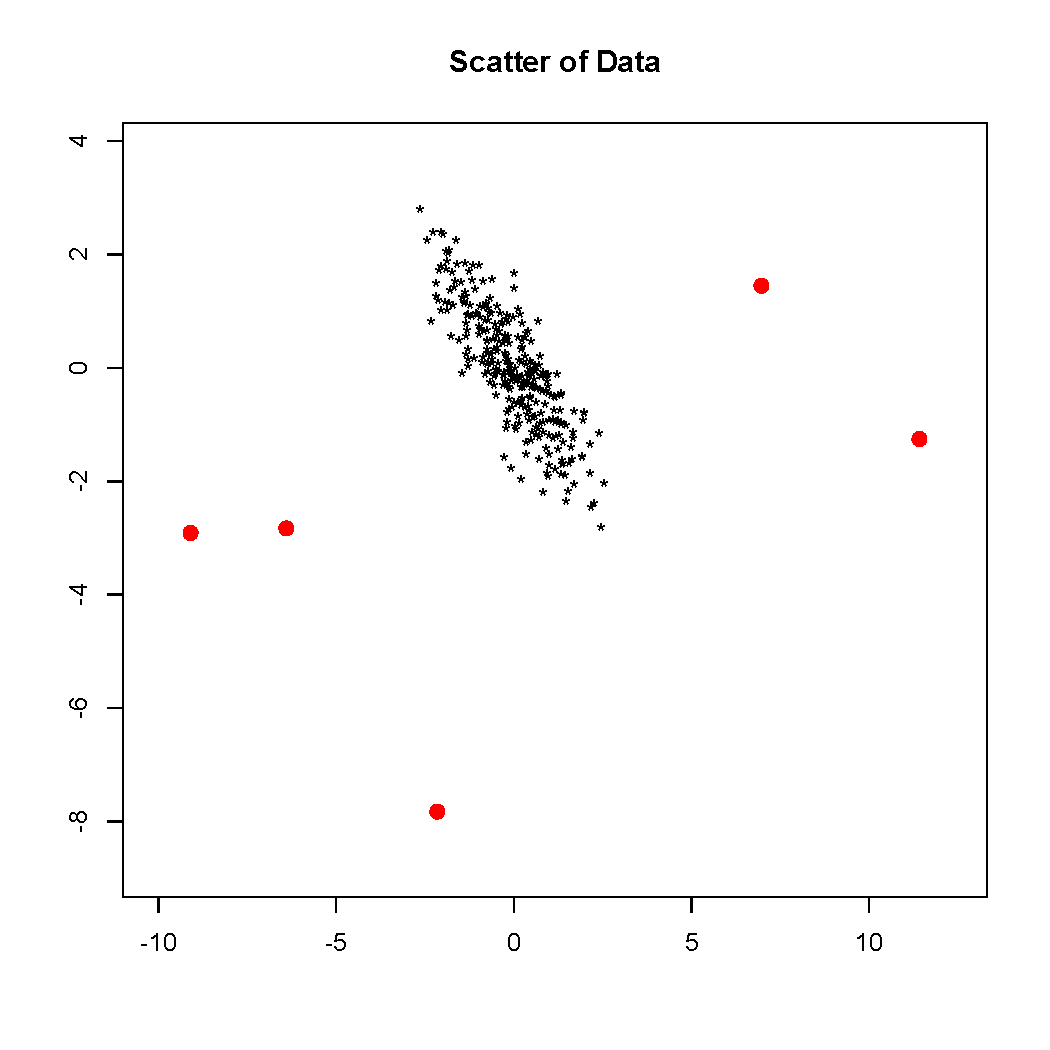
\includegraphics[width=0.45\textwidth]{../Plots_SC/WeightedSign_Scatter_02_27_19} &
%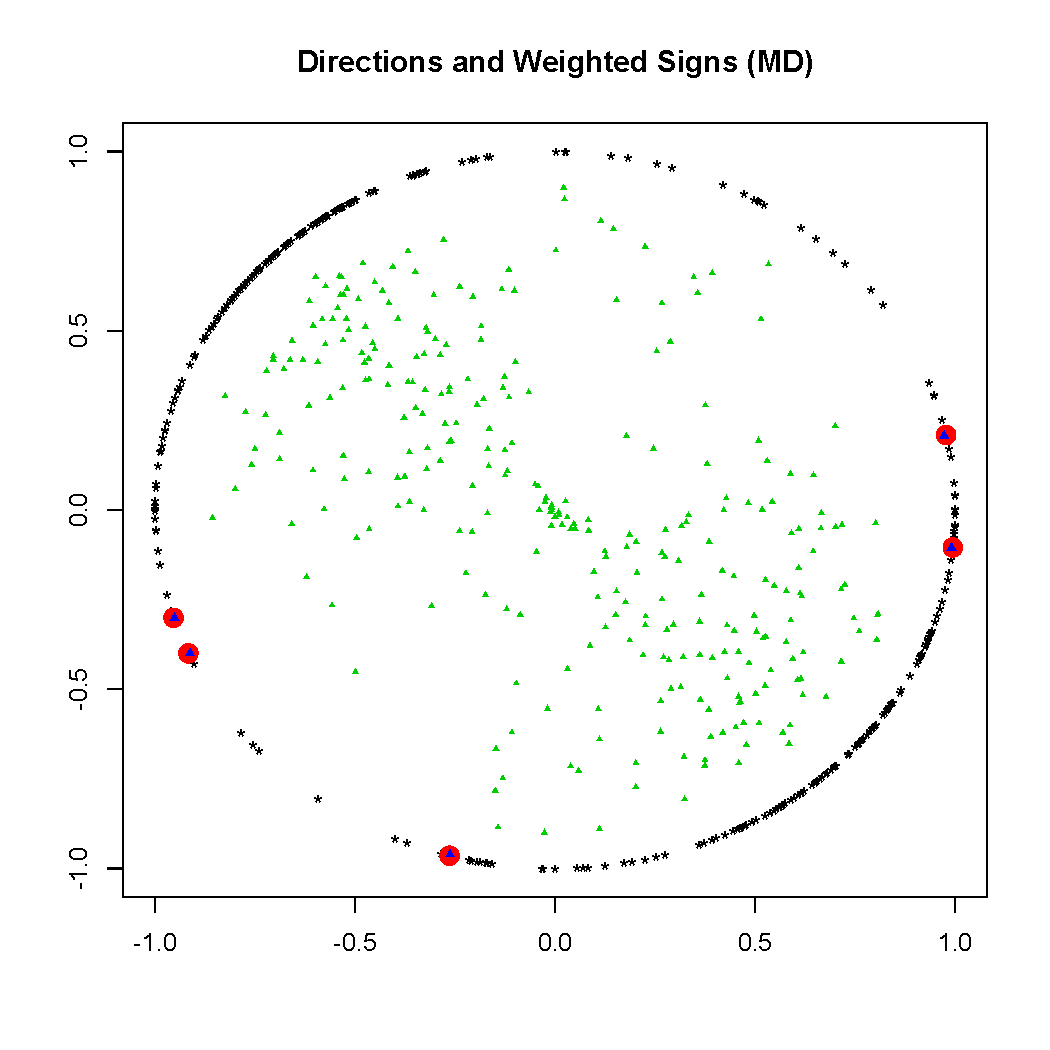
\includegraphics[width=0.45\textwidth]{../Plots_SC/WeightedSign_MD_02_27_19} \\
%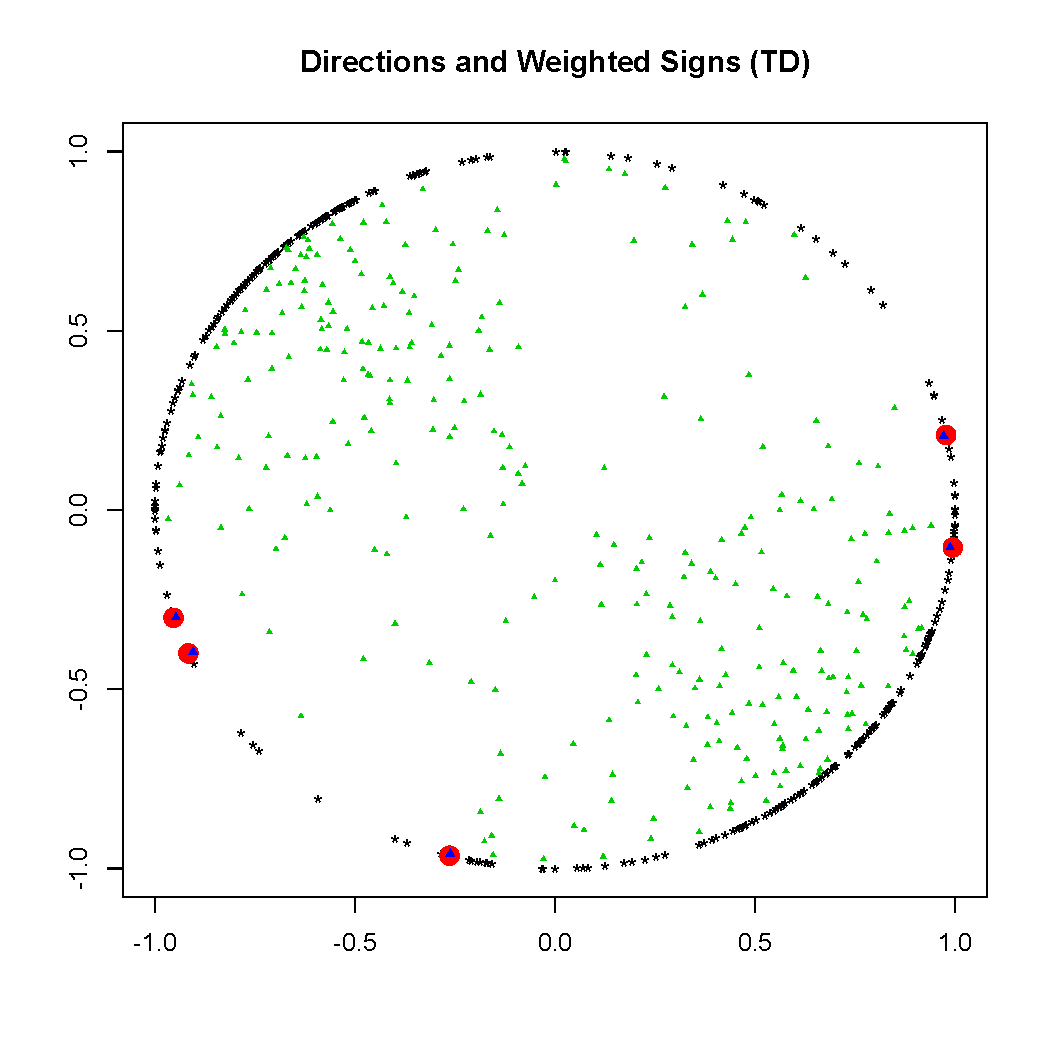
\includegraphics[width=0.45\textwidth]{../Plots_SC/WeightedSign_TD_02_27_19} &
%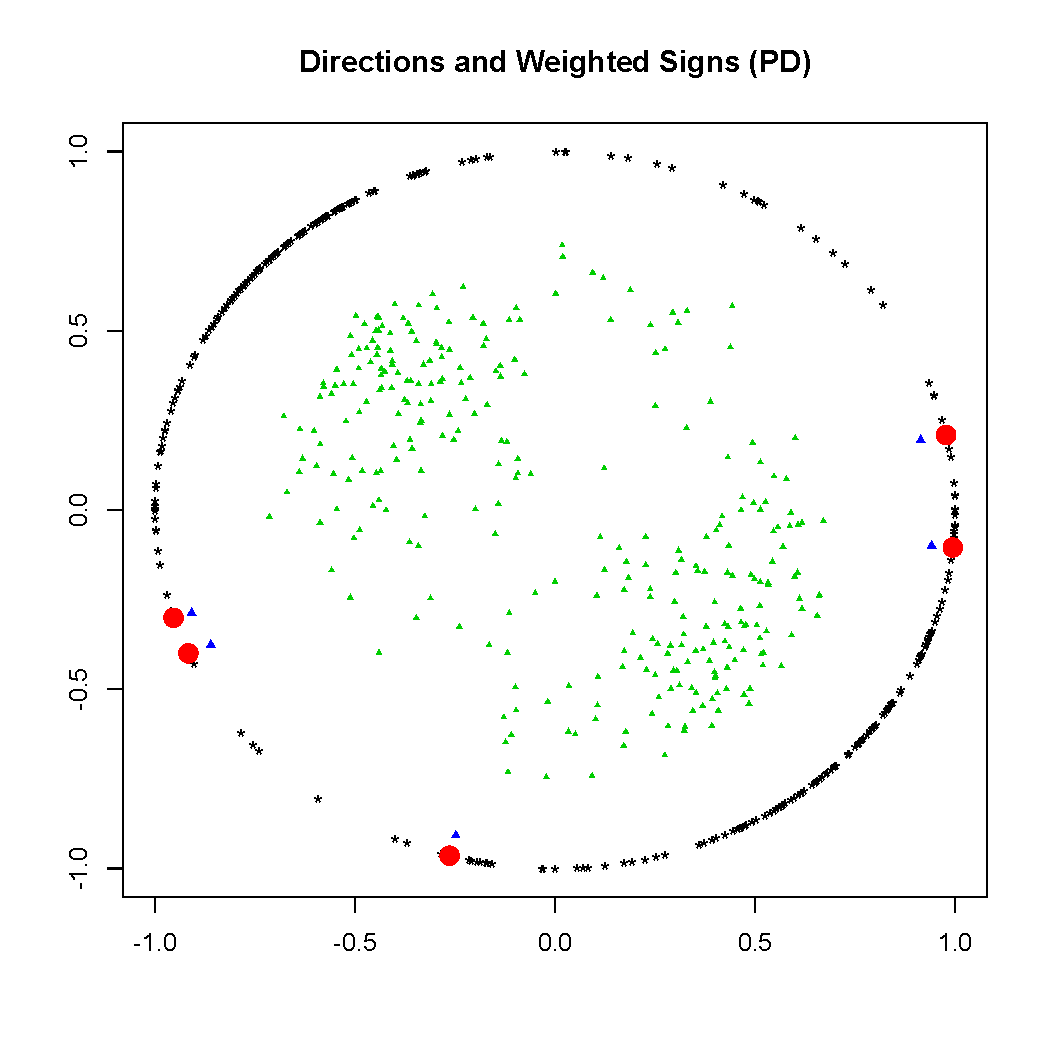
\includegraphics[width=0.45\textwidth]{../Plots_SC/WeightedSign_PD_02_27_19} \\

%%% These ones have sample size = 1e3, too large file for EJS
%\includegraphics[width=0.45\textwidth]{../Plots_SC/WeightedSign_Scatter_02_24_19} &
%\includegraphics[width=0.45\textwidth]{../Plots_SC/WeightedSign_MD_02_24_19} \\
%\includegraphics[width=0.45\textwidth]{../Plots_SC/WeightedSign_TD_02_24_19} &
%\includegraphics[width=0.45\textwidth]{../Plots_SC/WeightedSign_PD_02_24_19} \\
%\end{tabular}
\caption{
An illustrative bivariate scatter plot in the top left panel where the outliers are 
identified with red circles, 
and generalized signs from the same data (black points on the 
unit radius circle, outliers are red points) in the other panels. 
In the top right (bottom left, bottom right) 
panel, weighted signs from the same data with weights obtained using Mahalanobis depth 
(Tukey depth, projection depth respectively) are presented as green triangles 
(outliers are identified by blue triangles). 
}
\label{fig:Fig1}
\end{center}
\end{figure}
%\end{comment} 

We primarily focus on the task of \textit{robust dispersion/scatter estimation} and 
\textit{robust principal component analysis} in this paper. Figure~\ref{fig:Fig1} presents an illustrative example of bivariate data with outliers in the top left panel, where the outliers are marked with red points. In the 
other panels, the generalized sign values of the same data are presented as black points 
on the unit circle, with the outliers again marked with red points. Notice that the 
black points from either the top right or bottom panels have very similar eigenvector 
structure as the original data without the outliers. The green and blue triangles 
are examples of 
the proposed \textit{weighted sign} values: the top right (respectively, bottom left, 
bottom right) panels depict these values where the weights have been generated using 
Mahalanobis depth (respectively Tukey's half-space depth and the projection depth). The 
blue triangles are the weighted sign values of the outliers. Notice that the eigenvectors 
from the weighted signs also capture the pattern from the original data without the 
outliers.

There are two unknown quantities in the generalized sign function as defined in \eqref{eq:GSign}: $\mu$ and $\BF$, To estimate dispersion and its eigen-structure robustly, we must start with a robust estimator for $\mu$. In Section~\ref{Sec:WSQuantiles} we present the case for \textit{weighted spatial quantiles}, which can be defined and studied in very general spaces 
$\cX$. One special case of this is the {\it weighted spatial median}. As a location estimator, it has several interesting robustness properties and can be shown to be more efficient that some existing robust location estimators, thus making it a perfect candidate to estimate $\mu$. 
%On the other hand, setting $\BF$ as $\BF_X$, i.e. the distribution of $X$ has the clear interpretation of differentially weighting observations based on their inlyingness to the overall data distribution. This mirrors the context of how data depth has been used in the literature \cite{LiuPareliusSingh99, ref:DIMACS061_Serfling}. Due to this reason, we assume $\BF \equiv \BF_X$ for the rest of the paper. As and when required, we shall use sample versions of these quantities, stating the theoretical conditions for the corresponding approximation results to hold.

Following that, we restrict to the $\BR^{p}$ for fixed $p$, and present detailed discussions on our primary proposal for a  robust measure of dispersion in Section~\ref{Sec:WSDispersion1}, followed by a proposed \textit{ affine equivariant version} of it in Section~\ref{Sec:WSDispersion2}, robust estimation of eigenvalues and a third robust estimator for dispersion in Section~\ref{Sec:Eigen}, and a thorough study of robustness and efficiency using influence functions in Section~\ref{Sec:RE_Dispersion}. We then report multiple simulation-based numeric studies in Section~\ref{Sec:Simulation}, present several real data examples in Section~\ref{Sec:DA}, and concluding remarks in Section~\ref{Sec:Conclusion}.

In the rest of this paper, all finite-dimensional vectors are column vectors, and for a vector or matrix $a$, the notation $a^{T}$ stands for its transpose. The Gaussian distribution with mean $\mu$ and variance $\Sigma$ is denoted by $N (\mu, \Sigma)$. The identity matrix  is denoted by $\BI$, with or without a subscript to denote its dimension. The notations $A^{-1}, det (A), \lambda_{\min} (A), \lambda_{\max} (A)$ respectively stand for the inverse, determinant, minimum and maximum eigenvalues of a matrix $A$, whenever these are well-defined. For a scalar or vector valued random variable $Y$, $\BE Y$ denotes its expected value, while $\BV Y$ denotes its variance or covariance matrix.